\documentclass[10pt,a4paper,twocolumn]{scrartcl}
\usepackage[utf8]{inputenc}
\usepackage[english]{babel}
\usepackage[T1]{fontenc}
\usepackage{amsmath}
\usepackage{amsfonts}
\usepackage{amssymb}
\usepackage{graphicx}
\usepackage{setspace}
\usepackage[left=2cm,right=2cm,top=2cm,bottom=2cm]{geometry}

\usepackage{booktabs}
\usepackage[font=small]{caption}

\usepackage{hyperref}

\usepackage{natbib}
\bibliographystyle{alpha}
%\bibliographystyle{spr-chicago}
%\bibpunct[:\,]{(}{)}{;}{}{}{,}

\title{Reception of LGBT in Newspapers}
\author{Magdalena Bönisch \and Till Haubenreißer \and Maximilian Möller}
\publishers{\emph{Universität Leipzig, Introduction to Digital Humanities (Dr. Köntges)}}


\begin{document}
\onehalfspacing

\maketitle

{\small
\paragraph*{Abstract} For the last decades, there has been a rapid shift from discrimination and exclusion to integration and equality of lesbian, gay, bisexual, and transgender (LGBT) people. Based on articles of the New York Times, this work pursures the question whether there has been a shift within LGBT-related reporting as well. The two analyzed aspects of reporting are the manner how the journalist reports on LGBT-related events, and the topics within the articles. Sentiment analysis revealed that the how of reporting is constant over all newspaper articles. The sentiment is mostly determined by the newspaper genre. Nevertheless, topic modeling shows that different topcis are relevant in different times. The proposed hypothesis is that knowing the topic shift of some ``older'' LGBT term as \textit{homosexual} allows a projection to ``newer'' terms, e.g. \textit{transgender}.
}


\section{Introduction}
On September the 29th in the year 2016, California legalized as the first nation in the United States an all-gender restroom access law, which allowed people of all genders to use the former single-occupenced restrooms in public places \citep{Ring:2016}. According to that, there were a lot of articles in the newspapers dealing with this new law as a positive aspect and great LGBT-achievement. There were people discussion openly about the situation of transgender people, it was called a big step towards equality and LGBT was all in all a positively discussed theme in the news.

Thinking of the beginning of LGBT-popularity, there is an other atmosphere calling to mind. Only a few decades ago, there were a lot more harassment and discrimination against sexually other-orientated people. In many countries homosexuality was treated as a crime or a mental illness. Over the years, the LGBT-community has gained more and more attention. Comparing the situation not that many years ago with the mood today, there has been a big change. It is this change we are interested in. What has the LGBT-community achieved over the years and how is it shown in the media? What influenced a time? Can we make a future forecast according to the changes in the past?

As a good indicator of a timeperiod we determined the newspaper, as it is well known for representing local and global issues in an objective way. We have chosen the New York Times because it is an important and well known press with the intention to report unbiased. In addition, it has a good API to gather data with which we could work afterwards. On this basis, we were interested in two thing: How does the sentiment of the articles changes over the years? And what other topics show up accompanying LGBT search terms.

The first question is addressed by sentiment analysis \citep{Nasukawa+Yi:2003, Godbole+al:2007, Cambria+al:2013}. It is part of text analysis in the context of natural language processing and computer linguistics. While telling facts, a writer can still transmit his opinion and judgments or influence the reader by emotional talking or unbiased reporting. The sentiment analysis tries to identify the attitude of the writer towards the topic he is writing about and to evaluate it.

Topic modeling \citep{Wallach:2006, Blei:2012} meanwhile does not care about the `how' it is told, but more what the text is about. It is also part of the text analysis but while the sentiment somehow looks for the connotation of words, the topic analysis deals with the words themselves. Every text can be divided in some main-subjects it is dealing with. Manually, these subjects can be easily found by reading, clustering and brainstorming, but for a mass of data, an automatic solution has to be applied. We targeted a simplified approach of topic modeling based on automatic extraction of words significantly cooccurring with an LGBT-related term. Then, the topics were manually created based on these cooccurrences. Such a semi-automatic approach has the advantage that the clustering of cooccurrences is of high quality.

All in all, this project is about gathering data related to LGBT-topics across a huge timespan, finding topics and sentiments for the data and at least analyzing the change over time. Our goal is to find and portrait a significant change in the reporting on LGBT-related topics from 1850 to today, display the achievements in the rights and equality of LGBT-people and perhaps make a little prognosis about future changes according to the behavior we detected in the past.

The paper is structured as follows. In section \ref{sec:workflow}, the workflow as well as decisions concerning the implementation are elucidated. Section \ref{sec:underlyingdata} presents the data underlying the subsequent analyses described in the workflow. Section \ref{sec:results} shows the results for the sentiment analysis as well as for the simple topic model approach. After that, section \ref{sec:discussion} starts with technical and implementational comments to the current workflow. Furthermore, content issues are discussed. Eventually, ideas for future work are discussed. This thesis ends with a conclusion and a take-home message.

\section{Workflow \& Implementation}\label{sec:workflow}
In the following, the general workflow for analyzing the LGBT reception within newspapers is described. Subsequently, the concrete decisions concerning the implementation are addressed.

\subsection*{Workflow} The overall workflow is shown in Fig.~\ref{fig:workflow}. The upper part reflects the first step of collecting newspaper articles and creating a database. For each term from a predefined list of query terms, an HTTP request to the API of an online newspaper archive is sent. In this work, the Article Search API of the New York Times\footnote{\url{https://developer.nytimes.com/}} has been used as it provides access to articles published since its foundation in 1851 and thus enables an extensive time-dependent analysis. Furthermore, the returned JSON documents contain not only a URL to the actual article but also textual attributes like the lead paragraph and the publication date. The analysis is based on these text fields. Hence, no further call for the complete article is necessary. Since the access to the NYT API is limited per second and per day, the responses are parsed and stored into a MySQL\footnote{\url{https://www.mysql.com/}} database. A relational database allows a quick access to the data along with SQL as a powerful query language for data selection and summarization. By using the database, subsequent analysis is based on the whole corpus independent of the API. Furthermore, the proposed workflow is more flexible with respect to adding data from an additional newspaper archive since its response only has to be mapped to the scheme of the database while the analysis module (lower part of the workflow in Fig.~\ref{fig:workflow}) remains unaffected.

\begin{figure}
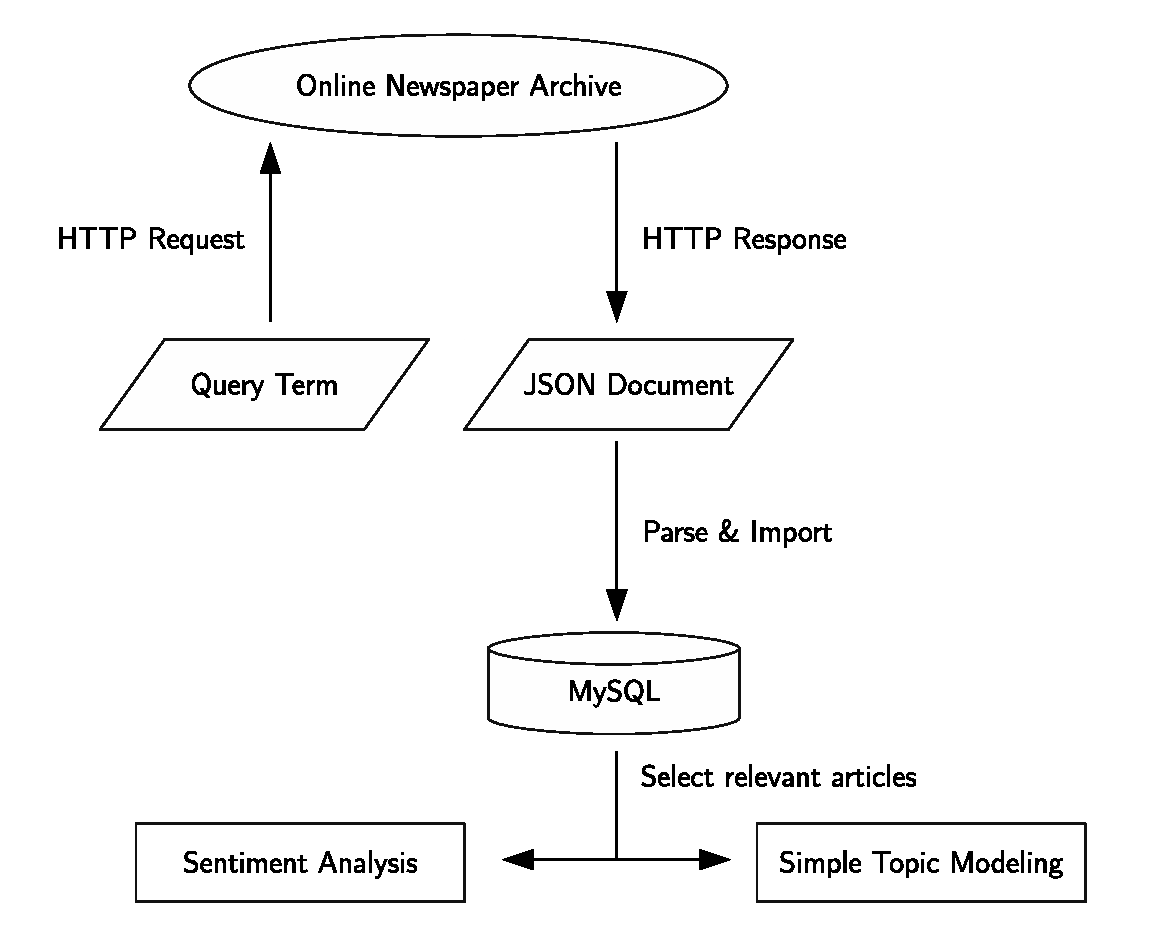
\includegraphics[width=\columnwidth]{figures/workflow_eps}
\caption{Workflow} \label{fig:workflow}
\end{figure}

The analyses are based on two dimensions: query term and time. Thus, the input of the sentiment analysis and the simplified topic modeling approach is a set of lead paragraphs containing the query term and contained in articles published at a certain time. For instance, such an input can be all lead paragraphs from the database which contain the word \textit{homosexual} and which were published in the 1990s.

The sentiment analysis assigns each sentence a vector of sentiment probabilities. We have considered five sentiments: \textit{very negative}, \textit{negative}, \textit{neutral}, \textit{positive}, and \textit{very positive}. For example, the vector \begin{center}
$v_s = \langle 0.2, 0.5, 0.1, 0.1, 0.1\rangle$
\end{center} describes the case that a sentence $s$ has a probability of $20\%$ for having a very negative sentiment, $50\%$ for having a negative sentiment, and $10\%$ for having a neutral, positive, and very positive sentiment, respectively. For the topic modeling, the joint occurrence of a target term together with another word (cooccurrence) is analyzed. Target terms are LGBT-related words, like the query terms.\footnote{The query terms are used for building an LGBT-corpus. But within this corpus it is possible to search for other terms than query terms as well. For instance, \textit{lesbian} is a query term as well as a target term. \textit{gay} is only a target term.} For each cooccurrence, its frequency and its significance is calculated. For instance, the cooccurrence \begin{center}
$c_\text{2010s} = \langle \text{bisexual}, \text{rights}, 31, \text{true}\rangle$
\end{center} means that within the lead paragraphs from 2010 to 2019, \textit{bisexual} and \textit{rights} occurred 31-times in the same paragraph and that this occurrence is significant. By clustering significant cooccurrences, the topics were manually created in order to yield high-quality topics.

\subsection*{Implementation} The whole workflow has been implemented in Java as a Maven\footnote{\url{https://maven.apache.org/}} project. The project is managed on GitHub.\footnote{\url{https://github.com/macksimiljan/lgbt-news}} It consists of one module for collecting and one for analyzing the data. The database is accessed by using the Java Database Connectivity (JDBC) API\footnote{\url{http://www.oracle.com/technetwork/java/javase/jdbc/index.html}}.

\paragraph*{Collecting Module} The used query terms are \textit{bisexual}, \textit{gay community}, \textit{homosexual}, \textit{lesbian}, \textit{transgender}, and \textit{transsexual}. However, the term \textit{gay} was not considered as a query term because it appeared too often in non-LGBT-related contexts, as a given name or surname, for instance. In order to obey the time limit of the NYT API, only one request per second was sent. Almost all requests ($95.4\%$) were successful. They returned a non-empty JSON object which was then inserted into the database. Failures of requests were due to denied access to the archive (HTTP 403) or gateway time-outs (HTTP 504). Because such failures were very rare, failed requests were not sent for a second time. All in all, the built corpus consists of $44,485$ articles, $93,7\%$ of which contain a non-empty lead paragraph on which the analyses are based.

The database models the mapping of query terms and keywords to articles. Keywords represent additional information on the articles such as associated persons, organizations, or geographical information. Approximately $75\%$ of all articles have at least one keyword. Moreover, an article has a URL which points to its HTML representation in two-thirds of the cases; otherwise the article is only accessible as a PDF document.\footnote{Older articles are archived as PDF not as HTML.} Further attributes are the publication date, the actual text type (for instance, article, interview, or biography), the headline, an abstract, the lead paragraph, and a snippet. Since the headline is very short, the abstract is missing for $62\%$ of the articles, and the snippet is mostly the same as the lead paragraph, the analysis is based on the lead paragraph. For the body of the article, the HTML representation of the article would have had to be requested and parsed.

\paragraph*{Analysis Module} Essentially, the analysis module of the Maven project comprises the sentiment and the topic model package. They both rely on the sentence extraction task. For a certain target term and a certain publication date, this task selects windows of sentences from the paragraphs in the database. Given a window size of 2, for instance, in addition to the sentence containing the target term, the two directly preceding as well the two directly succeeding sentences are extracted.\footnote{For the given corpus, a window size greater than 4 will have no difference to a smaller size since the paragraphs consists only of a few sentences. For instance, not more than 40\% of the paragraphs consists of two or more sentences.} For the sentiment analysis, we have chosen a window size of 0, i.e. only the containing sentence, and for the topic modeling a size of 1.  Both analyses depend on the natural language processing library Stanford CoreNLP\footnote{\url{http://stanfordnlp.github.io/CoreNLP/}}. This library contains annotators for tokenization, sentence splitting, part-of-speech tagging, and sentiment analysis. Since the sentiment annotator is based on the sentence structure, it is expected that it returns better results than approaches which only count the occurrences of particular negatively or positively connotated words or phrases while ignoring their syntactic context \citep{Socher+al:2013}. However, determining the sentence sentiment is a very time consuming operation. Therefore, we have chosen the minimal window size.

The simplified topic modeling approach consists of three steps: preprocessing, cooccurrence counting, and the statistical evaluation. The preprocessing is executed for the corpus only once. For all paragraphs, the contained words and their number of occurrence are determined. Stop words and numbers are excluded from this word statistics. The stop word list is based on \citep[p.533]{Manning+Schuetze:2003} whereas numbers are recognized by a regular expression. After having created the word statistics, it is possible to define the list of context words. A context word is a meaningful word which cooccurs with a target term. A word is assumed to be meaningful if it is not a stop word or a number and has a minimum frequency of 3. The frequency condition enforces that words being typographical errors are excluded from the analysis. After preprocessing, the word statistics consists of approximately $66\cdot 10^3$ word types and $1.2 \cdot 10^6$ word tokens.\footnote{Since we followed a simple approach, we did not run a lemmatizer. For comparison, the Oxford Dictionary counts about $200 \cdot 10^3$ (lemmatized) word types (inclusive stop words) in the English language \citep{Oxford}.}  $43.4\%$ of all words occur only once or twice. Thus, there are approximately $29\cdot 10^3$ context words.

In the next step, all cooccurences of a target word $w_\text{target}$ with one of the $n$ context words are counted in the paragraphs containing $w_\text{target}$ and published in a certain time span $t$. To yield the cooccurrences and their number, these paragraphs were tokenized and cleansed by removing all non-context words from the sentences and transforming the remaining words to lower case. For instance, the sentences \begin{center}\textit{The president argues for gay rights. He is tolerant.}\end{center} is mapped to \begin{center}\textit{president argues gay rights tolerant}\end{center} This sequence of words is used to built a context vector $v_t(w_\text{target}) = \langle c_1, c_2, \ldots, c_n\rangle$ for each $w_\text{target}$ and $t$ such that $c_i$ represents the (absolute) frequency of the cooccurrence of $w_\text{target}$ with the context word at list position $i$. Because cooccurrence is not a reflexive relation between two words, $c_i = 0$ if the context word at position $i$ equals $w_\text{target}$. In the example, assume that the list of context words $L$ consists of six words: \begin{center}$L =  [\text{argues, gay, president, rights, tolerant, usa}]$\end{center} Depending on the chosen maximum distance $d_\text{max}$, the context vector $v_t(\text{gay})$ for the target word \textit{gay} is built. Let $d_\text{max}$ be 2, then there can be not more than $d_\text{max} - 1 = 2 - 1 = 1$ word between the target word and its cooccurrence partner. This yields the context vector \begin{center}$v_t^1(\text{gay}) = \langle 1, 0, 1, 1, 1, 0\rangle$\end{center} because every word except for \textit{usa} cooccurs with \textit{gay} exactly once. For $d_\text{max} = 1$, only the direct neighbors of \textit{gay} are considered resulting in the context vector \begin{center}$v_t^2(\text{gay}) = \langle 1, 0, 0, 1, 0, 0\rangle$.\end{center} Studies suggest that the average sentence length in written prose is between 20 and 25 tokens, for instance \citep{Sichel:1974}. The maximum distance $d_\text{max}$ is not sentence-sensitive, i.e., it ignores sentence boundaries. Nevertheless, as the paragraphs are only a few sentences, there is a maximum distance $d'_\text{max}$ such that for all distances greater than $d'_\text{max}$ the number of cooccurrences is the same. Fig.~\ref{fig:distance} shows this for the count of cooccurrences with \textit{gay} in the 2010s. The number of all cooccurrences as well as the number of significant cooccurrences converge to 7650 and to 2300, respectively. These values are reached for a maximum distance greater than 56 (not shown in the figure). Tests with further target words lead to similar results. However, the smaller the maximum distance, the more semantically connected the words of the cooccurrence are expected to be. Choosing a great distance, the cooccurrences can connect words which are probably in different sentences. Since the sentence boundary is a semantic boundary as well (each sentence represents a logical statement on its own), a great maximum distance results in cooccurrences which might include words that should not be interpreted as being semantically connected. Thus, we run the program with a maximum distance of 6 and of 14 for all target terms and times. For  $d_\text{max} = 6$ ($d_\text{max} = 14$), approximately $67\%$ ($85\%$) of all cooccurrences and $40\%$ ($67\%$) of all significant cooccurrences are detected. 


\begin{figure}
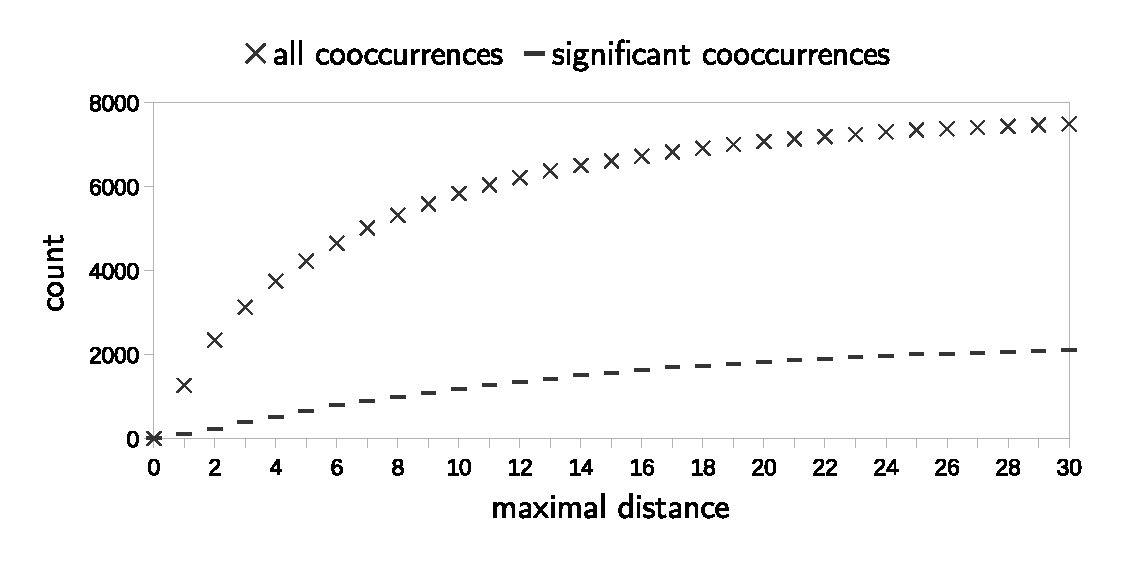
\includegraphics[width=\columnwidth]{figures/distance_eps}
\caption{Convergence of the number of cooccurrences.} \label{fig:distance}
\end{figure}

The last step is the calculation of significant cooccurrences. Following \citep{Bordag2008, Manning+Schuetze:2003}, three significance measures were implemented: mutual information, log-likelihood, and t-score. For some test data, the t-score yields the best results. Let $n$ be the number of context words, $n_\text{t}$ and $n_\text{c}$ the number of occurrences of the target term and of a context word, respectively, and $n_{\text{t}\text{c}}$ the count of the cooccurrence of $w_\text{target}$ and $w_\text{context}$, then the t-score is defined according to Eq.~\ref{eq_tscore}.

\begin{equation}
\text{t}(w_\text{target}, w_\text{context}) = \frac{n_{\text{t}\text{c}} - \dfrac{n_\text{t} \cdot n_\text{c}}{n^2}}{\sqrt{n_{\text{t}\text{c}}}} \label{eq_tscore}
\end{equation}

 Consequently, a cooccurrence is defined as significant if it passes the t-test for $p = 0.005$. Additionally, all cooccurrences were selected occurring more often than on average in order to get further hints for topics. 



\section{Underlying Data}\label{sec:underlyingdata}

Choosing the underlying data and retrieving it correctly was a crucial part of our work. Not only we had to choose terms that are most used in an LGBT context but also we had to filter the content for relevant articles in our case. There are a lot of terms but not all of them are useful for analysis. In the end we came up with 6 useful terms that delivered enough data to be relevant. These are: \textit{bisexual}, \textit{gay community}, \textit{homosexual}, \textit{lesbian}, \textit{transgender} and \textit{transsexual} making in sum $44,485$ articles and a mean of $95.38\%$ of all articles with these search terms in the NYT database. 

Why did we choose those words as our data foundation? Firstly they are diverse. They cover a wide variety of alternative gender models without going to much into detail. Secondly they are very prominent. As already said if there aren't enough articles the relevance decreases. Thirdly they cover all timespans researchable via the API, the NYT was founded in 1851. Some of the terms were used very early while others gained importance just in the last time. The number of articles per decade for a given query term is shown in Fig.~\ref{fig:bisexual}, Fig.~\ref{fig:gayCommunity}, Fig.~\ref{fig:homosexual}, Fig.~\ref{fig:lesbian}, Fig.~\ref{fig:transgender}, and Fig.~\ref{fig:transsexual}.


\begin{figure}
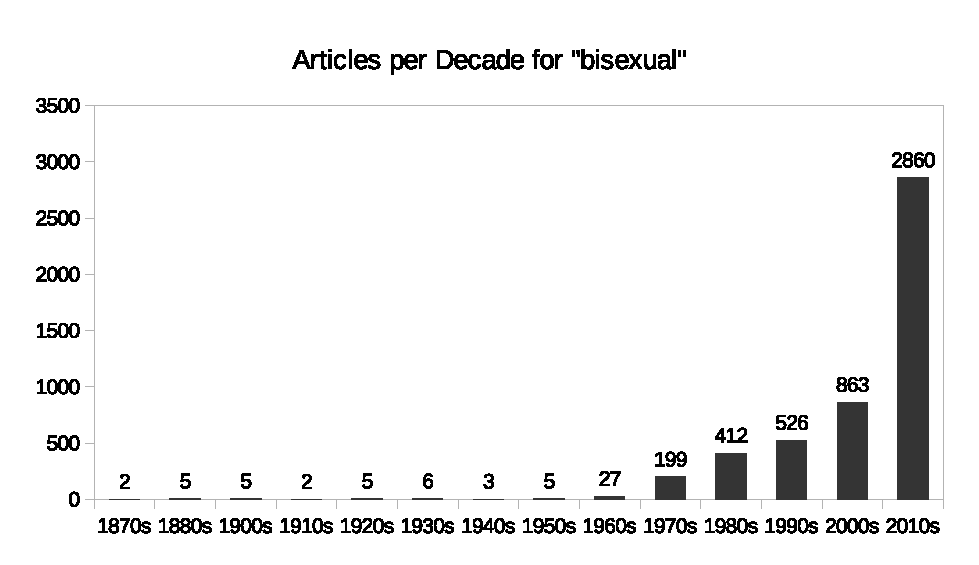
\includegraphics[width=\columnwidth]{figures/bisexual_decade}
\caption{Number of articles for \textit{bisexual}.} \label{fig:bisexual}
\end{figure}

\begin{figure}
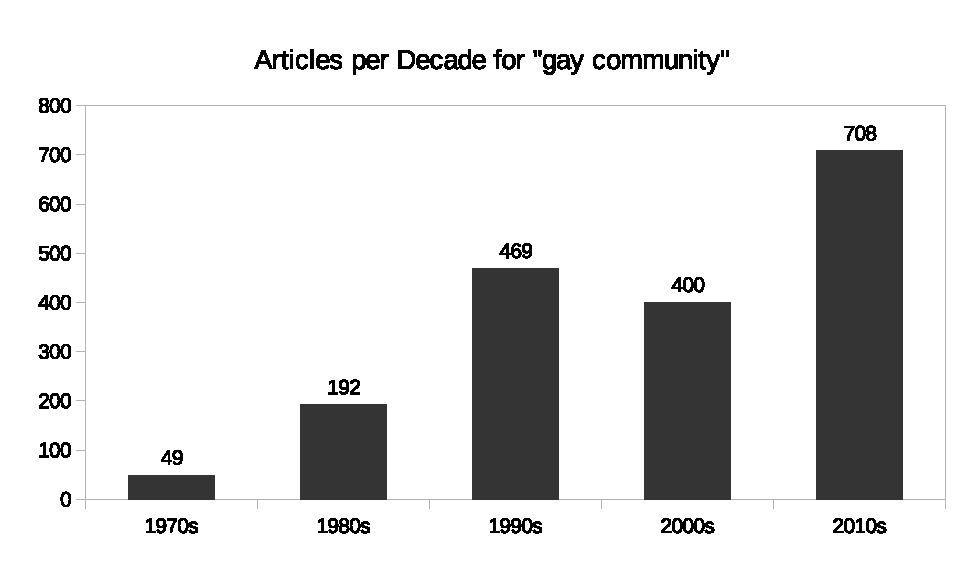
\includegraphics[width=\columnwidth]{figures/gayCommunity_decade}
\caption{Number of articles for \textit{gay community}.} \label{fig:gayCommunity}
\end{figure}

\begin{figure}
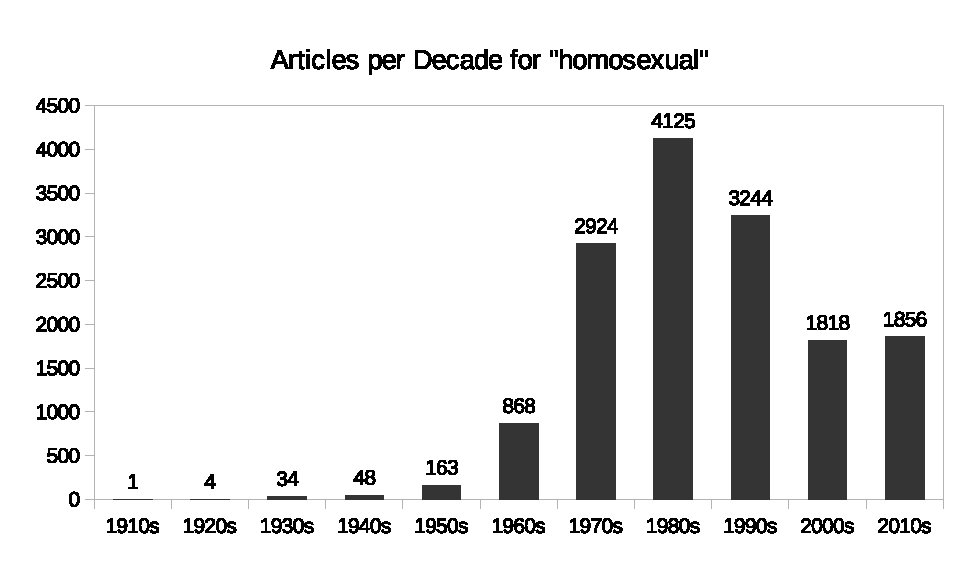
\includegraphics[width=\columnwidth]{figures/homosexual_decade}
\caption{Number of articles for \textit{homosexual}.} \label{fig:homosexual}
\end{figure}

\begin{figure}
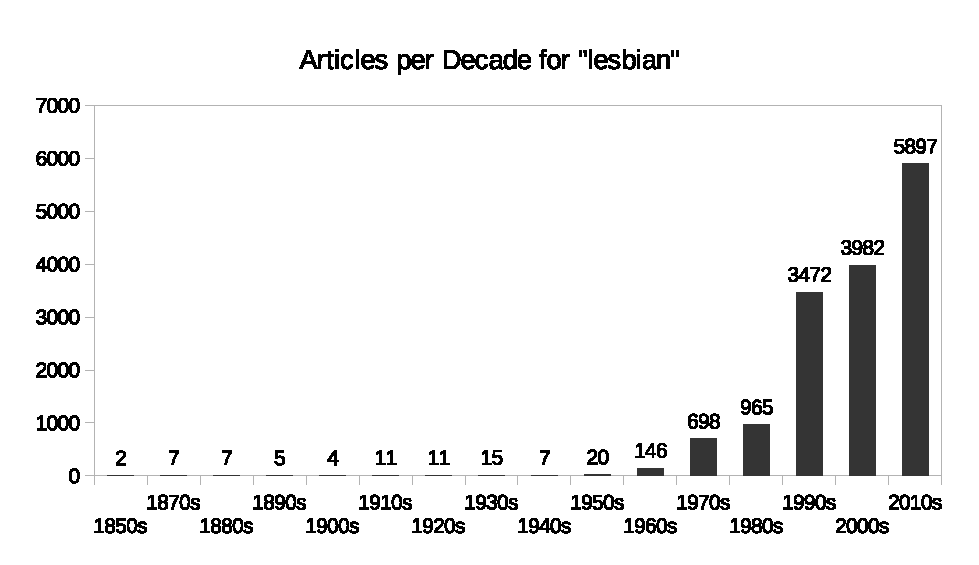
\includegraphics[width=\columnwidth]{figures/lesbian_decade}
\caption{Number of articles for \textit{lesbian}.} \label{fig:lesbian}
\end{figure}

\begin{figure}
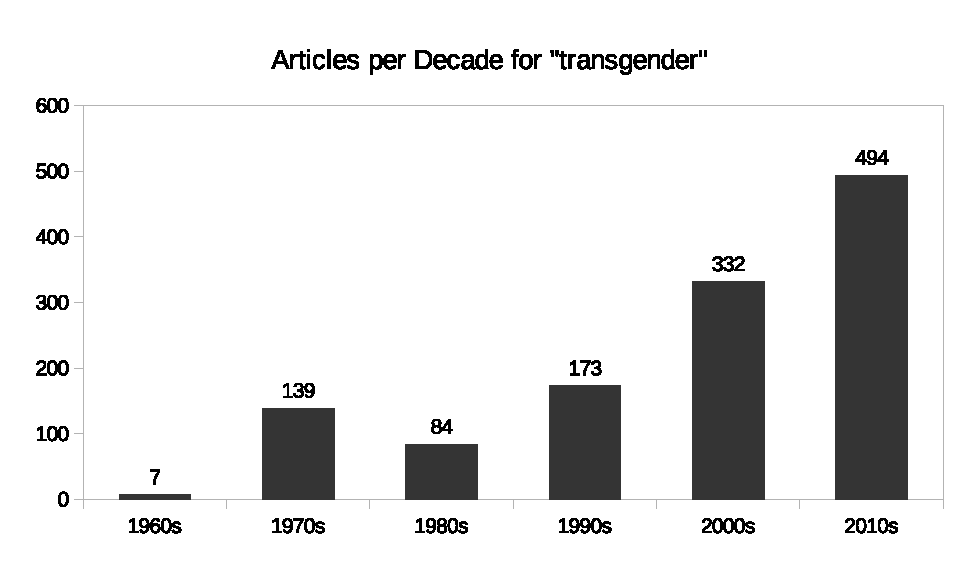
\includegraphics[width=\columnwidth]{figures/transgender_decade}
\caption{Number of articles for \textit{transgender}.} \label{fig:transgender}
\end{figure}

\begin{figure}
\includegraphics[width=\columnwidth]{figures/transsexual_decade}
\caption{Number of articles for \textit{transsexual}.} \label{fig:transsexual}
\end{figure}


Why didn't we choose other words that are even more prominent for example \textit{gay}? This has several reasons. Let's stay with the word \textit{gay}. It doesn't have an exclusive meaning just in LGBT context. It also means \textit{happy} meaning we would have gotten lots of articles that have nothing to do with our research topic because it was used in the sense of \textit{being happy}. Another reason is, that gay is also a quit common name or part of a name. 
There are a lot of other terms we did not use due to reasons like not enough relevance, usage in specific context or not given researchability. 

One thing we thought about analyzing but eventually decided against was a visualization of geographical information. Only 37\% of all articles have an assigned geographical location. Thus, we doubted the relevance of such a visualization.

So we have a lot of articles but that is just one part. The other part is sentiment analysis and topic modeling to really get something out of the texts. For sentiment analysis, we focused on the 1980s and 2010s because for both decades have many articles and we wanted to compare two times which we expected to have very different reports on LGBT. An extended sentiment analysis for other decades would have gone beyond the scope of this work.

The analyses are based on the \textit{lead paragraph} attribute of each article. 94\% of the articles have such a paragraph. Nevertheless, it is not necessarily the case that a lead paragraph assigned to a certain query term actually contains this query term. For instance, although there are $4,920$ `bisexual' articles in the database, only 570 of these articles have a lead paragraph containing \textit{bisexual}. Nevertheless, there are 1495 lead paragraphs containing \textit{bisexual} in the whole database. The difference emerges from the fact that the NYT API does not search within the lead paragraph but only in the headline, byline and body. As our textual analyses are based on the lead paragraph, the count of target terms in all paragraphs in the database is shown in Tab.~\ref{tab:dataBasis}.

Because one target word can occur in more than one lead paragraph, paragraph duplicates are expected. Within the database, 28\% of all lead paragraphs occur more than once. Duplicates are eliminated during selection of paragraphs from the database.

\begin{table}
\centering
\caption{Size of the data basis.} \label{tab:dataBasis}
\begin{tabular}{lrr}
\toprule
term	 & \#articles & \#paragraphs\\
\midrule
bisexual &  $4,920$ & $1,495$\\
gay			& $-$ & $10,392$\\
gay community & $1,818$ & 377\\
homosexual  & $15,086$ & $5,263$\\
lesbian & $15,249$ & $5,086$\\
queer  & $-$ & 162\\
transgender  & $6,138$ & $2,973$\\
transsexual  & $1,229$ & 279\\
\bottomrule
\end{tabular}
\end{table}

A brief glance at the article type reveals that most articles (in a broader sense) are news ($56.1\%$). Articles (in a narrow sense) and reviews are about $10.2\%$ in each case. Approximately $6.0\%$ of all articles are actually blogs. All other types, e.g. letter, interview, or editorial, occur less than $5\%$. No further analyses are based on the type information.

Finally, the created corpus has been compared with the Google Books corpus accessed by the Ngram Viewer.\footnote{\url{https://books.google.com/ngrams}} Fig.~\ref{fig:google} shows the relative frequency for LGBT-related terms in American English books. The upper diagram contains our query terms while the lower one visualizes the occurrence of other LGBT terms. Very prominent is the maximum of \textit{lesbian} (red line) in the late 90s. A closer look at our corpus reveals that there is a similar maximum for \textit{lesbian} but some years earlier. Since newspaper articles are assumed to reflect events more immediately than books, we concluded that it is the same maximum. However, the decrease of \textit{bisexual}, \textit{homosexual}, and \textit{lesbian} since the late 90s, can be only confirmed for \textit{homosexual} in our corpus. The steady increase of \textit{transgender} and \textit{transsexual} is attested in both corpora. The lower diagram shows the frequency of \textit{gay} and \textit{queer}. The characteristic of both terms is that they are present in the literature long before the upper terms occur. Furthermore, as soon as the upper terms emerged, the frequency of \textit{gay} and \textit{queer} decreased while an increase can be observed since the 90s. The hypothesis is that these terms changed their meaning in an infrequent phase from 1940 to 1990 and since that they have been frequently used as LGBT terms.

Overall, the comparison with the Google Books corpus shows that we can assume our data to be representative. Furthermore, it supports the decision to exclude \textit{gay} and \textit{queer} from the query terms as their behavior is different to the actual query terms.

\begin{figure*}
\centering
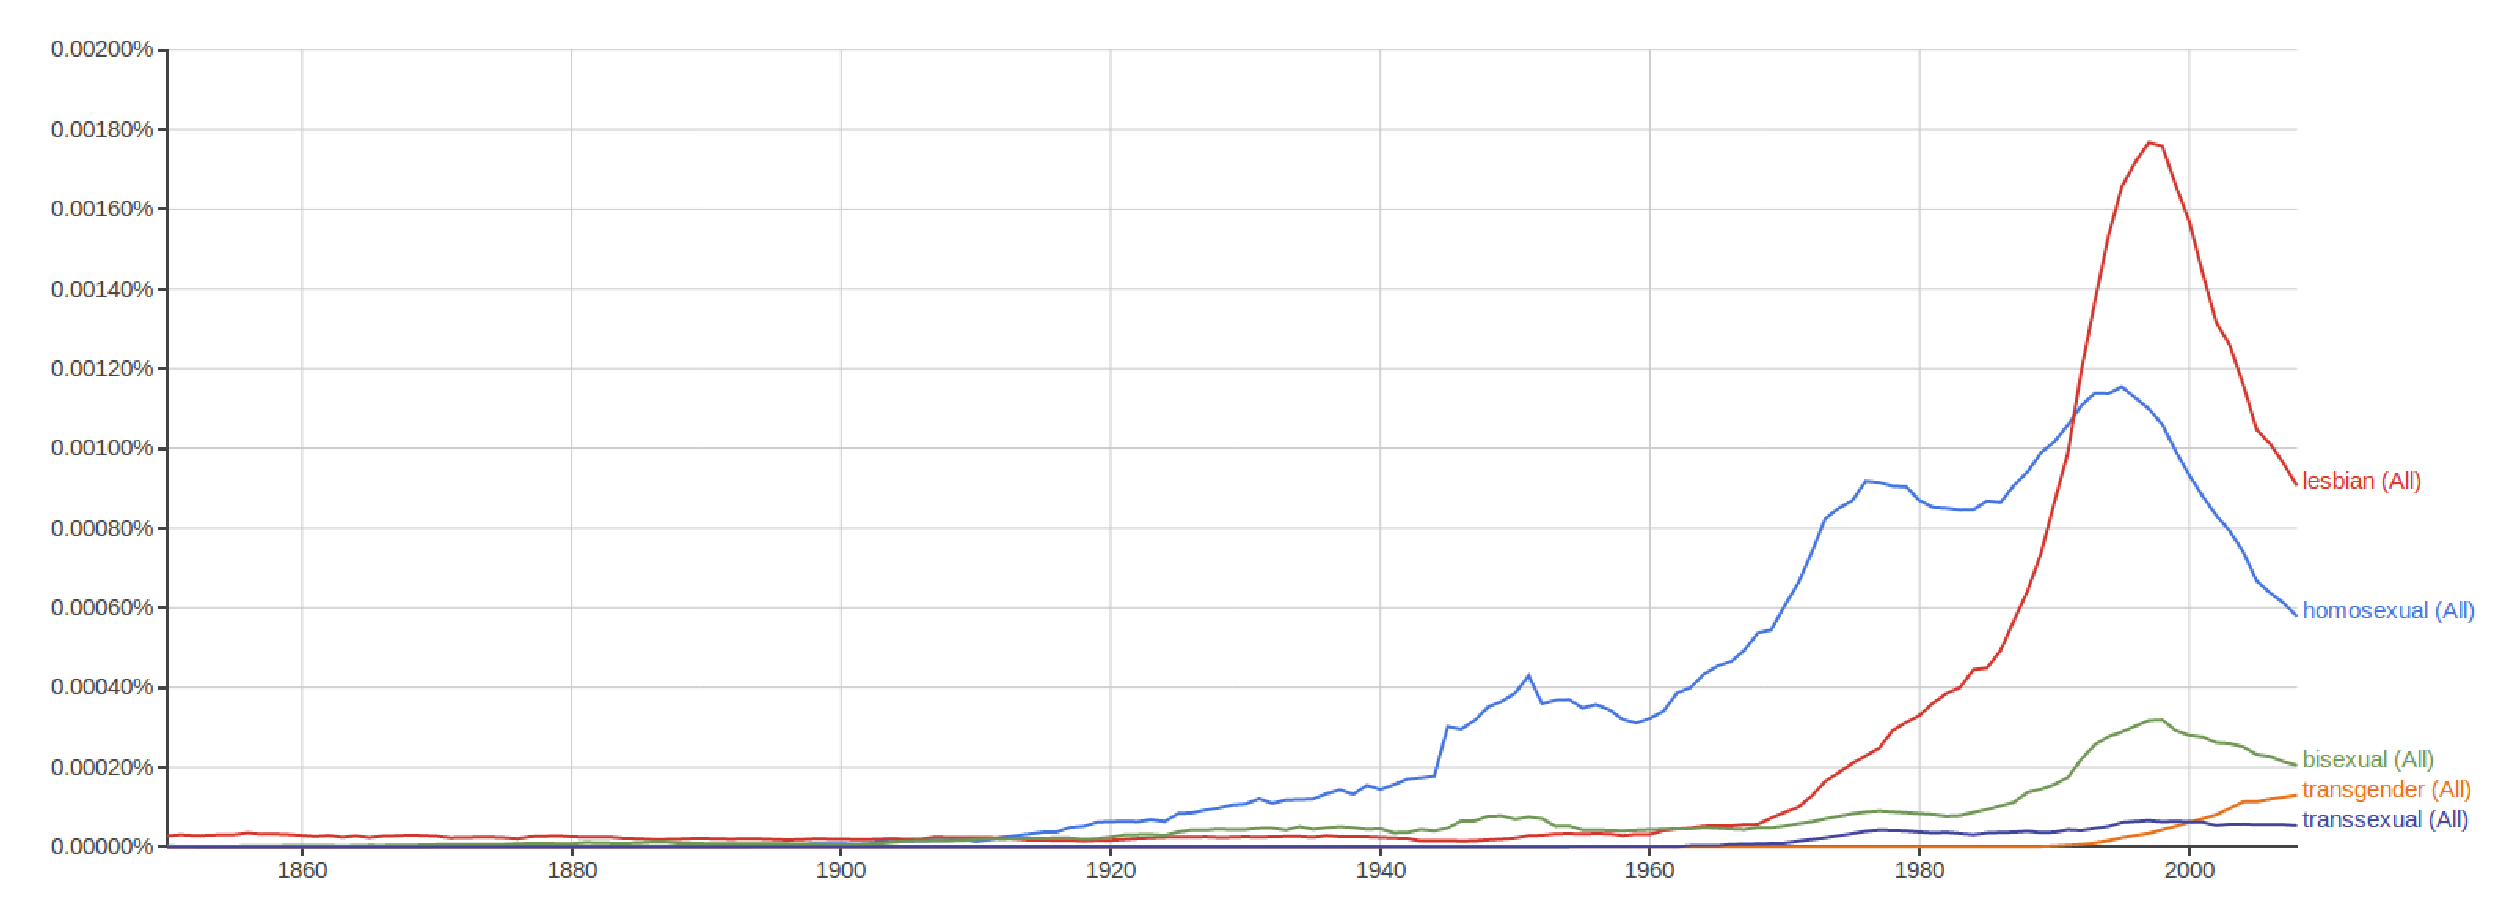
\includegraphics[width=\textwidth]{figures/google_queryterms}

\vspace*{1cm}

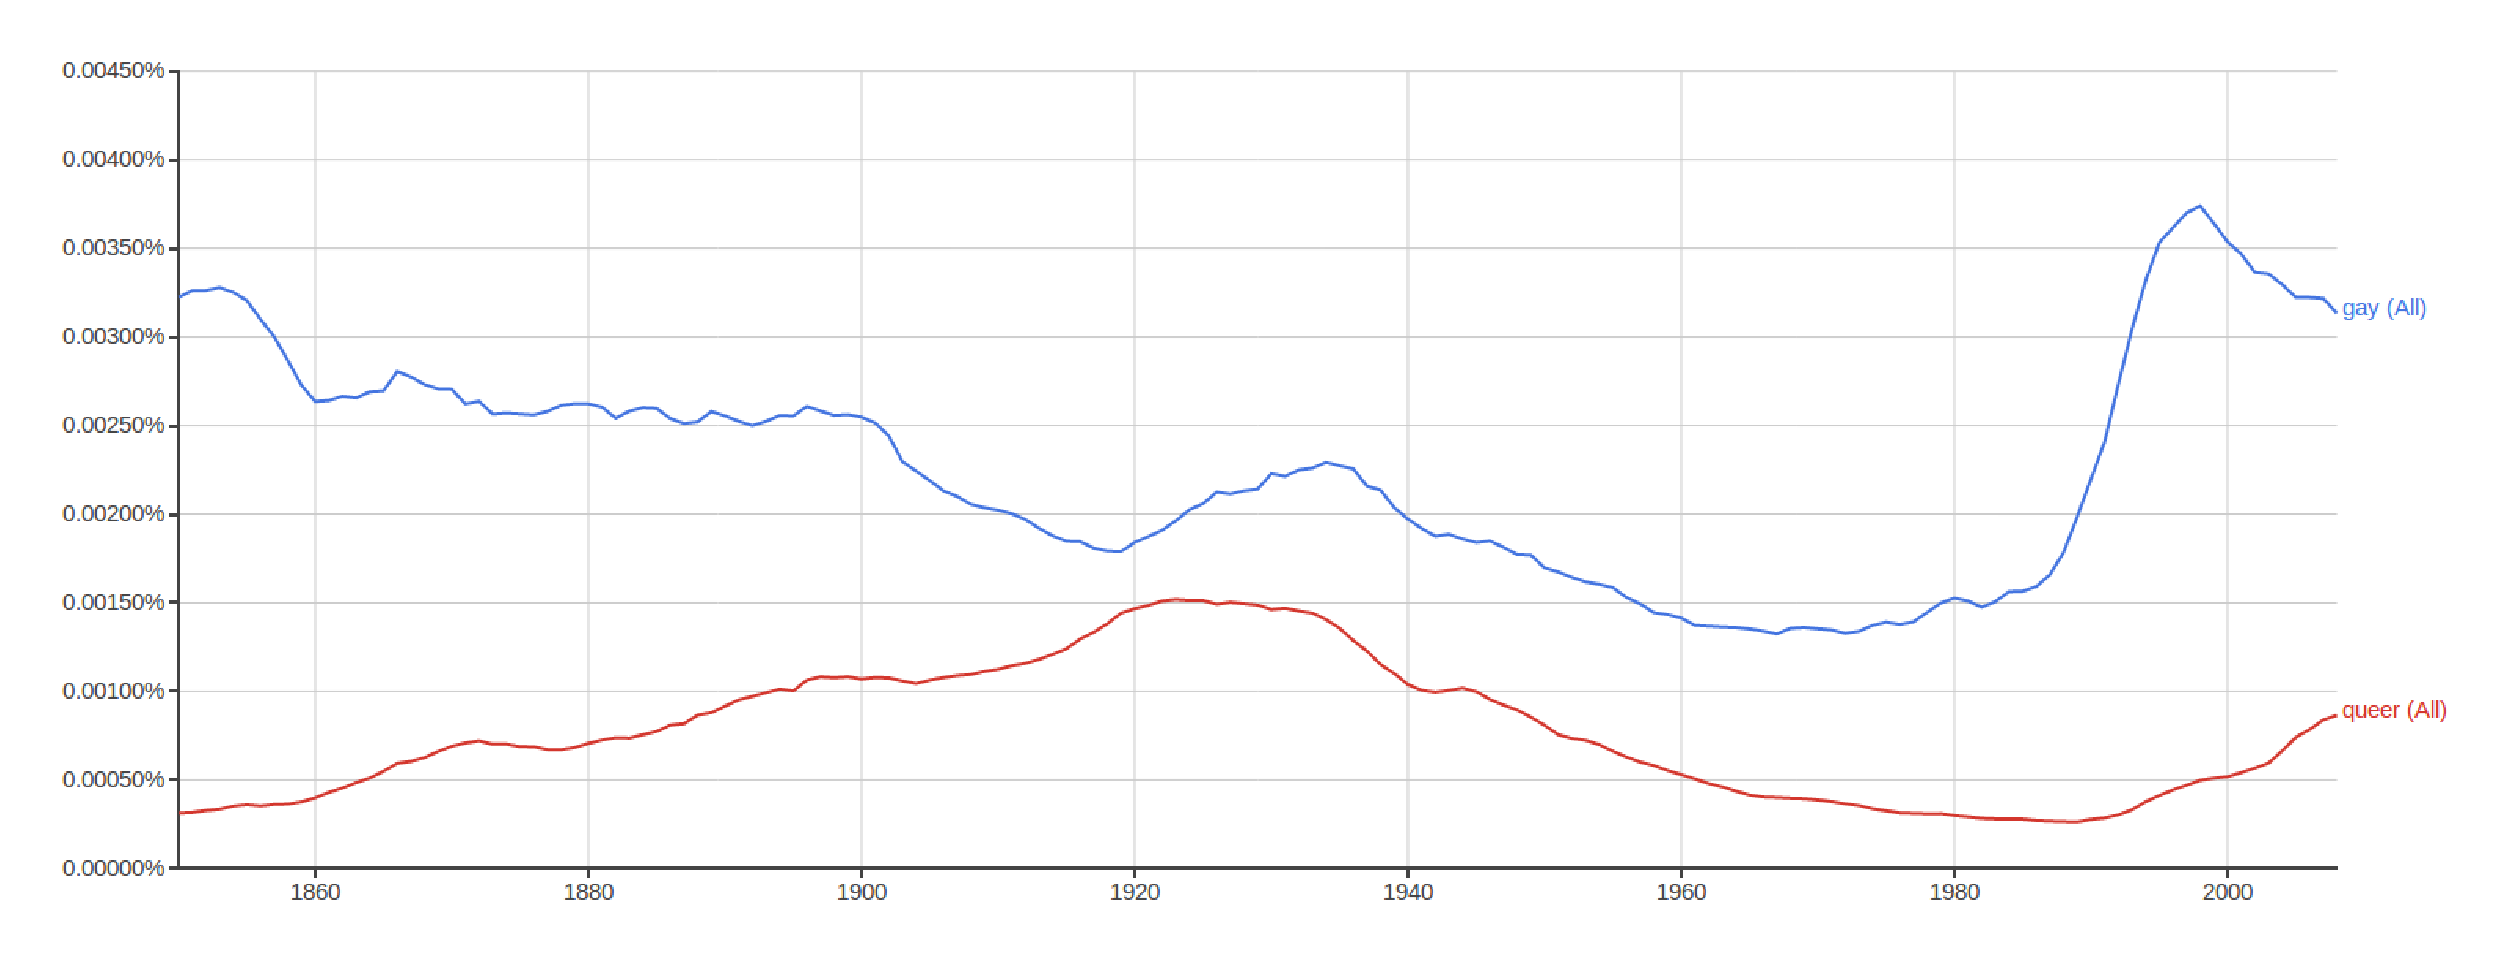
\includegraphics[width=\textwidth]{figures/google_others}
\caption{Google Books Ngram Viewer: LGBT-related terms.} \label{fig:google}
\end{figure*}



\section{Results}\label{sec:results}



\subsection{Sentiment Analysis}

For the sentiment analysis, we compared the sentiments of sentences containing a target word from early newspaper articles (1980s) with ones from current articles (2010s). Furthermore, the sentiment results among the target words were compared. All in all, there were no significant differences within these conditions. On average, 85\% of all sentences are assigned the sentiment \textit{negative}. \textit{very positive} is determined for less than $0.1\%$ of all input sentences of the sentiment analysis. The frequencies of the other sentiments are in the range of 2\% to 8\%. All standard deviations are smaller than $1.5\%$ percent points.

There are two explanations for the minimal differences between the conditions. First, the sentiment distribution mainly depends on the genre, i.e., all newspaper articles are written in the same manner. Each article reports the events objectively and with no significant attitude of the author. The mostly negative sentiments are a side-effect of the newspaper ductus. Second, there has been (and still is) a negative reporting for all LGBT news.

To test both explanations, further articles were extracted from the NYT article archive as a baseline for expected positive sentiments. These articles were football news as we assumed that reporting on football is positive. The distributions of sentiments over sentences for LGBT terms and the football baseline are shown in Fig.~\ref{fig:sentiment1}. The \textit{football} data show indeed more positive sentiments than LGBT news. However, about 70\% of all sentences\footnote{For \textit{football}, the input of the sentiment analysis comprises 125 sentences.} have still a negative sentiment. Thus, we have concluded that negative sentiments are very likely due to the newspaper genre.

\begin{figure}
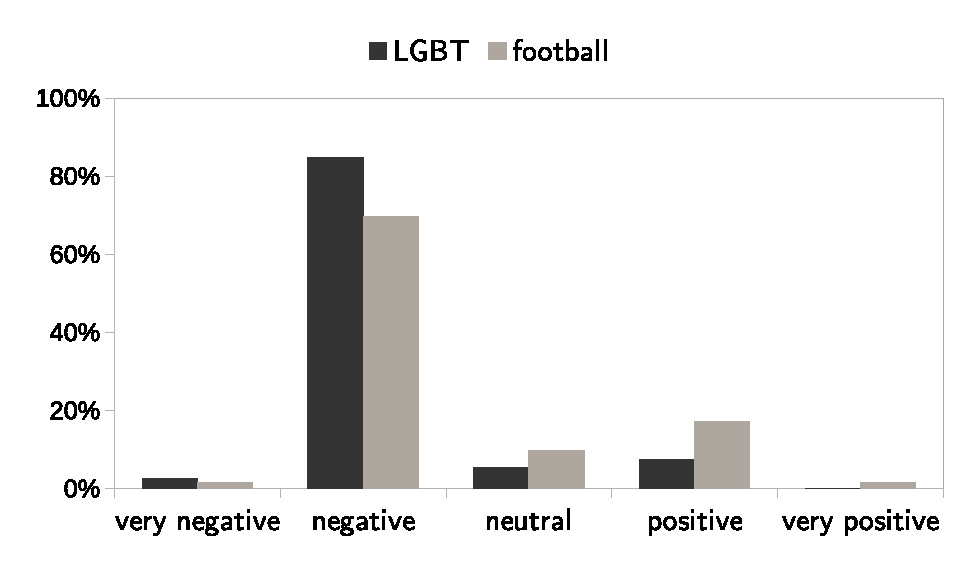
\includegraphics[width=\columnwidth]{figures/sentiment1}
\caption{Frequency of sentiments.}\label{fig:sentiment1}
\end{figure} 


It is important to bring to mind that the output of the sentiment analysis is not a sentiment category in the first place. Rather, an vector of probabilities is returned.  Hence, it might be possible that the competition between sentiments was very close. For the sentiment vector $v_{s_1} = \langle 0.0, 0.46, 0.1, 0.44, 0.0\rangle$, for example, the decision for \textit{negative} and against \textit{positive} is very close since the difference in the probabilities is marginal. However, for the vector $v_{s_2} = \langle 0.0, 0.8, 0.1, 0.1, 0.0\rangle$ it is clear that the sentence $s_2$ has a negative sentiment.


\begin{table*}
\centering
\caption{Average sentiment probabilities.} \label{tab:prob}
\begin{tabular}{lccccc}
\toprule
 & very neg. & negative & neutral & positive & very pos.\\
\midrule
LGBT, 1980s & 16.9\% & 51.0\% & 20.5\% & 8.7\% & 2.8\%\\
LGBT, 2010s & 16.5\% & 51.9\% & 19.8\% & 8.8\% & 3.0\%\\
football &  13.6\% & 44.8\% & 21.3\% & 14.4\% & 5.9\%\\
\bottomrule
\end{tabular}
\end{table*}

But also on the underlying probability level, the results are equal for all conditions. The averaged probabilities are summarized in Tab.~\ref{tab:prob}. For the articles from the 1980s (2010s), the standard deviation is less than $1.3$ ($1.5$) percent points. Since the expected probability of each sentiment is $^{100\%}/_{5} = 20\%$  for a random distribution, a probability for \textit{negative} greater than $40\%$ can be seen as a clear result. Nevertheless, there is still a certain probability of about $20\%$ that such sentences are \textit{neutral} instead of \textit{negative}. A similar pattern emerges for \textit{football}.

To summarize, the sentiment analysis showed no differences between target terms or different times. A detailed evaluation of the precision of the sentiments is presented in the discussion.

\begin{figure*}
\begin{minipage}{0.48\textwidth}
\includegraphics[width=\columnwidth]{figures/topic_lgbt}
\caption{Incidences of \textsc{lgbt-related terms}.} \label{fig:topic_lgbt}

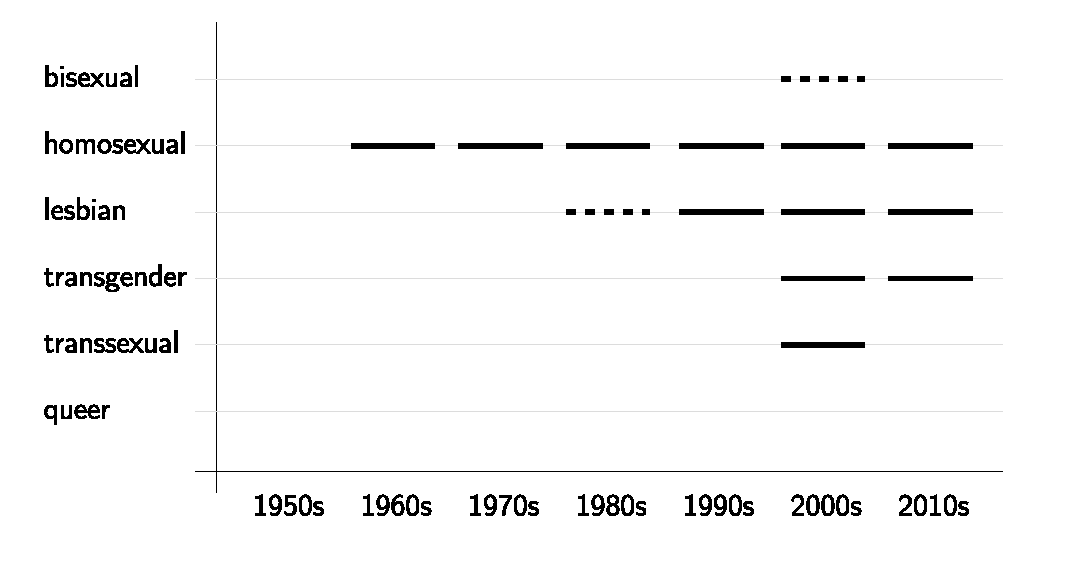
\includegraphics[width=\columnwidth]{figures/topic_rights}
\caption{Incidences of \textsc{righs/law}.} \label{fig:topic_rigths}

\includegraphics[width=\columnwidth]{figures/topic_violence}
\caption{Incidences of \textsc{discrimination/violence}.} \label{fig:topic_violence}

\includegraphics[width=\columnwidth]{figures/topic_identity}
\caption{Incidences of \textsc{sex/identity}.} \label{fig:topic_identity}

\includegraphics[width=\columnwidth]{figures/topic_military}
\caption{Incidences of \textsc{military}.} \label{fig:topic_military}
\end{minipage}
\hfill
\begin{minipage}{0.48\textwidth}
\includegraphics[width=\columnwidth]{figures/topic_religion}
\caption{Incidences of \textsc{religion}.} \label{fig:topic_religion}

\includegraphics[width=\columnwidth]{figures/topic_activists}
\caption{Incidences of \textsc{activists/movement/org.}.} \label{fig:topic_activ}

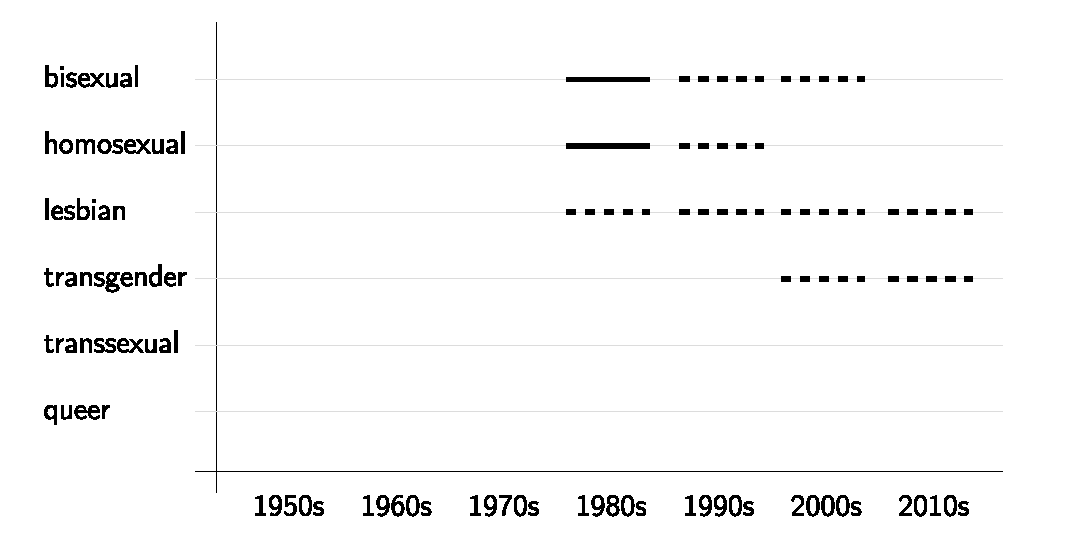
\includegraphics[width=\columnwidth]{figures/topic_health}
\caption{Incidences of \textsc{health}.} \label{fig:topic_health}

\includegraphics[width=\columnwidth]{figures/topic_tv}
\caption{Incidences of \textsc{television/film/other media}.} \label{fig:topic_tv}

\includegraphics[width=\columnwidth]{figures/topic_school}
\caption{Incidences of \textsc{school}.} \label{fig:topic_school}
\end{minipage}
\end{figure*}

\subsection{Simple Topic Modeling}
For all LGBT terms, ten main topics could be determined. First, the topic \textsc{lgbt-related terms} describes the occurrence of a target term with other LGBT-related terms. Fig.~\ref{fig:topic_lgbt} shows whether a target term appears in contexts with this topic at a certain time. Dashed lines indicate that the topic is present but not very often whereas a solid line denotes that the topic is very frequent. The topics of particular target terms are discussed below.

Secondly, \textsc{rights/law} is a very frequent topic. It contains court decisions or governmental statements to LGBT issues. Its incidences are shown in Fig.~\ref{fig:topic_rigths}. Third, an important topic is \textsc{discrimination/violence}, see Fig.~\ref{fig:topic_violence}. It covers not only discriminating utterances but also bodily harm and murder. The topic \textsc{sex/identity} covers the question of social and psychological identity. It is shown in Fig.~\ref{fig:topic_identity}. The next two topics \textsc{military} and \textsc{religion} describe the acceptance of LGBT people within a certain social environment, namely the military, Fig.~\ref{fig:topic_military}, and the religious institutions, Fig.~\ref{fig:topic_religion}. In addition, the topic \textsc{activists/movement/organizations} occurs whenever it is reported on people standing up for LGBT rights and equality. Its incidences is visualized in Fig.~\ref{fig:topic_activ}. Another topic, especially frequent in the context of AIDS in the 1980s, is \textsc{health}, see Fig.~\ref{fig:topic_health}. The topic \textsc{television/film/other media} is assigned to articles talking about LGBT people in movies, series or other media. The incidences of this topic are shown in Fig.~\ref{fig:topic_tv}. Finally, many articles deal with the acceptance and integration of LGBT people in educational institutions. The occurences of this topic \textsc{school} are presented in Fig.~\ref{fig:topic_school}.

Comparing the appearance of different topics in the target terms across the year, an overall movement can be observed: The first target term to recognize different topics is \textit{homosexual}. It occurred in the context of \textsc{discrimination/violence} and \textsc{rights/law} even before the other target terms were popular in the media. In the 1970s, with the first appearance of LGBT-related topics, other LGBT terms appeared in the newspapers. Besides some specific topics like surgery (\textit{transgender}) or marriage (\textit{homosexual}), there is one growing LGBT-movement after the 70s which can be found in nearly all of the terms. So by now the less known parts of LGBT, as for example bisexual, queer or transgender, have only a small popularity and are rarely mentioned separately. Roughly sixty years ago, the term homosexual was rarely mentioned in the press. By regarding its development, we can hope, that in the future the other LGBT terms will follow its lead: emerging as a standalone topic with own problems and discussions, raising awareness over the years and in the end becoming ``normal'' -- an accepted and equal part of the society. Additionally, the tendency can be seen that \textit{homosexual} has had to struggle most intensively with these topics. Other LGBT-related terms are attested with the topics for a shorter time. For instance, while \textsc{religion} was a crucial topic for \textit{homosexual} in the 70s and 80s, \textit{lesbian} and \textit{transgender} have no such intense confrontations.

In our opinion, it is a positive and theory-supporting fact that the smaller terms who are part of the big LGBT-mass nevertheless distinguish in small details and particularities. For example, \textit{lesbian} is a term dealing not much with the topic \textsc{military} because of the small number of women in the army. Furthermore \textit{transsexual} often deals with \textsc{sex/identity} because it is a big question in changing gender and personality. In this way we can see that these terms are not only parts of the LGBT topic, but begin to become an own, individual topic.

\paragraph*{Homosexual} According to the target term \textit{homosexual} the change over time was very well observable. Homosexuality was the first non-heterosexual orientation which rose to public awareness. Until the 19th century, there were strict laws against homosexual relationships all over the world, which disappeared very slowly and gradually. The simple topic modeling is based an articles dating back to the middle of the 20th century. For earlier published articles, not enough data has been available. The articles were grouped by their publication date. Each group covers a decade and has been evaluated independently. In the 50s, just a few words were encountered, but all of them can be sorted into the topic \textsc{discrimination/violence}. While we still found a lot of words matching that context, a new topic arose in the 60s, which should stay across the following years and gain more and more importance: \textsc{righs/law}. There were a lot of articles about new governmental decisions and developments in the gay rights. That can be agreed with the fact, that in the 60s more and more countries decriminalized sodomy or homosexuality itself, so for example, Illinois was the first federal state of the USA to decriminalize sodomy in 1962. But nevertheless it still was a time of hate and discrimination of homosexuals, who gained more and more popularity. This rising of awareness persisted in the following decade and led to the appearance of more and more topics, e.g. \textsc{television/film/other media}: movies about homosexuality or with openly homosexual actors. Beside the rights and the discrimination, there were reports about the identity of homosexuals and activism groups supporting the rights and interests of the gay community. According to the increasing prominence, the church began to encounter the gay community, because homosexuality was seen as being incompatible with religious beliefs or the bible. Religious organizations were formed and acted against the homosexual movement. In addition, this time was the beginning of the popularity of the LGBT and it were not only the homosexuals about which was reported but other sexual orientation, as for example bisexuality came to the fore.

The 80s were a heavy setback for the LGBT-community as it was the time of the AIDS-epidemic, for which the homosexuals were blamed as a vector of diseases. It was a hard time and the newspaper were marked by reports of death, illness and the epidemic itself. So it was the AIDS-epidemic which mainly moved this decade (\textsc{health}), accompanied with a few reports about groups of activists supporting the homosexuals and discrimination they had to face.

After the epidemic was kept at bay, another topic occupied the homosexual movement: the marriage. In 1989, Denmark was the first country worldwide to allow a same sex union and in the 90s a lot of nations followed their example. This is reflected in the newspapers: There was a big popularity in the topics \textsc{sex/identity} (with focus on identity issues), \textsc{righs/law}, \textsc{activists/movement/organizations} (with focus on groups and demonstrations), and as well in the topic \textsc{marriage}. The latter topic is especially relevant for the target term \textit{homosexual}. But there were still discrimination accompanying this achievement of equal rights, which could be seen in the topics. Another question popping up these times were the permission to serve in the army as homosexual man. The \textsc{health}-topic abated, while the general awareness of LGBT-topics expanded and the homosexuals showed more and more popularity in movies and the media in general.
The marriage question was the last big problem to be solved in the history of LGBT. In the following decades, there popped up some smaller changes in law all over the time. The whole group of LGBT raised more and more awareness while discrimination still existed but decreased in comparison to the objective discussions about identity, sex and family. Homosexuality gained importance in the educational system and all in all has become a more and more equal part of the society over the years. Big questions are solved and one can hope that other LGBT-related topics will integrate as good as this old controversial subject in human history.

\paragraph*{Bisexual} As seen in the subject of homosexuality, other LGBT-related subjects firstly appeared in the 70s. In this first decade bisexuality was only mentioned on the edge of homosexual topics, but in the 80s it gained big popularity. Being known for the AIDS-epidemic, the 80s were a hard time for the homosexuals – but also for the bisexual orientated people. Those were accused of being the transmissioner of the illness even more than the only homosexual orientated gay community. As being bisexual they were seen as the medium between the homosexuals and heterosexuals and in this way being the reason that the `illness of the homosexuals' affects the heterosexual orientated people. Because of this, bisexuality was mentioned a lot in articles about AIDS in the 80s, health and death were put into context with homosexuals and intravenous drug-users as those are the other transmission groups of the epidemic.

After the epidemic, the bisexuals are mainly mentioned in LGBT-related contexts. They are also well known in the movie area as actor or in films dealing with LGBT topics, and bisexuality becomes a topic in schools and universities.

Concluding it can be said, that the term bisexual is more like a follower in LGBT topics: It is often mentioned in coherence with other LGBT subjects, but apart from the popularity around the AIDS-epidemic, it is less of a standalone theme and more a part of the big LGBT-movement.

\paragraph*{Lesbian} Overall it can be said firstly that data for the term \textit{lesbian} concerning topic modeling is available from the 70s onwards. Further on what is obvious is that some topics, for example \textsc{health}, \textsc{religion}, or \textsc{military}, never have played a big role in a lesbian context. \textsc{rights/law} quickly rises to great importance and prominence as well as \textsc{activists/movement/organizations}, though there is more change in it than in \textsc{rights} over the course of time. Related terms of LGBT have a slightly higher relevance in the earlier data but it then decreases. The quite low prominence of \textsc{health} could be on one side linked to the overall silencing of the topic in everyday live and on the other side to the slightly lesser risk of infection through injuries by sexual intercourse. In the case of \textsc{military} it is probably due to the relatively low percentage of women in the army as whole of which are just another small percentage lesbians. \textsc{religion} cannot be explained for sure. The high relevance of \textsc{rights/law} as well as \textsc{activists/movement/organizations} could very well be linked to the feminist movement which became popular in 1968. Terms related to \textit{violence} can be found but have compared to other terms in each decade a fairly low relevance. Why also\textsc{sex/identity} with focus on identity is overall low could be explained by the different opinions among the lesbian community but that is just an idea and it could have very well other reasons. As seen also in the discussion for sentiment analysis in subsection~\ref{subsex:contentIssues}, \textsc{television/film/other media} has a relatively great importance among the lesbian community.

\paragraph*{Transgender} Although the term \textit{transgender} emerged in the late 1960s \citep{Oliven:1965}, it occurs in the underlying corpus with a significant topic not until the 1990s, namely \textsc{lgbt-related terms}. The reason is that there are no lead paragraphs for earlier articles. In the 2000s, many topics are connected to \textit{transgender}. \textsc{school} is not only relevant because of the general issue of integration but also because of various articles about the Harvey Milk High School, a high school designed for LGBT people. Newspapers started to report on the identity question of transgender people and as it is seen by the social surroundings. Court decisions are relevant for transgender issues as well (\textsc{rights/law}). Discrimination merges in different areas, for instance housing.

In the current decade, \textit{transgender} has similar topics as other LGBT groups: \textsc{military}, \textsc{religion}, \textsc{discrimination/ violence}, etc. Nevertheless, are some special topics. Such topics concern the usage of bathrooms, surgeries, treatment of transgender people in prison, or the acceptance of transgender children as boy scouts.

\paragraph*{Transsexual} As for transgenders, the question of identity is very important to transsexuals as well. This topic emerged in the 1990s and was intensively discussed in the 2000s. Additionally, \textsc{rights/law} was also an influential topic those days. Nowadays, articles are published which deal with transsexuals in movies and series. For equality, it is reported on transsexual roles and actors. Interestingly, the surgery topic only occurred for \textit{transgender} but not for \textit{transsexual} although the transition from one sex to another is strongly related  to hormones or surgical procedures.

\paragraph*{Queer} For \textit{queer}, the only significant topic besides \textsc{lgbt-related terms} is \textsc{television/film/other media} in the 2000s. Most articles reported on two famous television series: \textit{Queer Eye For the Straight Guy} (premiered 2003) and \textit{Queer as Folk} (2000-2005). Note that \textit{queer} was only a target term but no query term such that less results are expected.


\section{Discussion}\label{sec:discussion}
First, implementational issues and technical challenges of the current workflow are discussed. Second, the discussion focuses on the evaluation of the results. Finally, proposals for future investigations are pointed out.

\subsection{Implementation Issues}
In order to compare the reception of LGBT-related terms in different newspapers, it is necessary to integrate further newspaper articles into the database. Especially for The Guardian\footnote{\url{http://open-platform.theguardian.com/}}, the integration into the database is no problem since the Guardian API returns less information than the NYT API, e.g. no publication date or lead paragraph. At the same time, this is a problem because the only information is the web URL to the article. Thus, in order to get the publication date and textual information, the workflow has to be extended by a further request for receiving the HTML page of the full article as well as by a parser for extracting relevant information from this HTML document. As soon as such an extension has been implemented, it can be used to get the full article also from the NYT archive. The full article body would enable a more comprehensive topic modeling. Attention should be paid that the Guardian API provides only access to publications dating back to 1999.

In addition, enriching the database by further articles and other newspapers will weaken the current semi-automatic approach. A larger data set will no longer allow to manually evaluate the cooccurrences in order to find topics. Thus, the topics have to be created automatically as well.

A general problem with the newspaper archive APIs is that the access is limited. Assume that there are $150 \cdot 10^3$ articles for a certain query term as it is the case for \textit{gay} in the NYT archive. Since the NYT API allows requesting only $10\cdot 10^3$ articles per day, collecting the whole result set would take 15 days. The same amount of articles is no problem for the Guardian API where $250\cdot 10^3$ articles can be requested per day.\footnote{The Guardian allows $5\cdot 10^3$ calls per day and a maximum amount of 50 articles per call.} Additionally, only the first 1200 articles can be addressed within requests to the NYT API. Consequently, in order to get all articles, each call should not return more results than this number. In our workflow, the publication date was restricted in order to obtain an appropriate result set size.

In the present paper, sentences were treated differently. On the one hand, sentences were assumed to be important semantic units. Thus, the sentiment analysis was only executed for the sentence containing the target word. On the other hand, sentence boundaries were ignored for the simple topic model. The underlying argument is that in order to extract the topic in which the target word occurs, it is not only worthwhile to look at the sentence but to consider the context of that sentence as well. Nevertheless, this argument can be also applied to the sentiment analysis. Thus, increasing the window size for sentiment analysis should be evaluated in further investigations. Then, the information on coocuccrences and sentiments can be extended by the distance from the target word. Cooccurrences along a great distance may be less informative as direct neighbors. In addition, the sentiment of the sentence containing the target word has a larger weight then the one of other sentences. An outstanding issue is the aggregation function when combining the results of different distances.

The evaluation of the cooccurrences has revealed that there are still a lot of `un-meaningful' words, for instance \textit{only}, \textit{some}, \textit{recent} but also \textit{people} and \textit{group}. Such words make it harder to evaluate cooccurrences. Thus, the stop word list should be expanded by \textit{only} and others. Alternatively, a part-of-speech tagger can be used instead of the stop word list. Then, cooccurrences are only considered for particular part-of-speech, e.g. for nouns and verbs. Furthermore, too generic words (\textit{people}) should be excluded from the context words as well. 


\subsection{Content Issues}\label{subsex:contentIssues}
Working on the \textbf{sentiment analysis} we had a lot of problems to deal with. In order to test the Stanford Library, we manually evaluated the sentiment analysis of the articles of the years 2010 to 2017 containing the target term \textit{transgender}, but the results were not exactly what we were looking for: More than 80\% of our test data has been recognized as negative. We took a closer look and evaluated the `negative-connotated' sentences. Firstly, we had to identify what the sentiment means: Does it describe the author's attitude towards the topic or is it more the connotation of the sentence and its words itself? Per definition it should be the attitude of the writer towards his topic, but for normal a journalist should write unbiased and objective which is not in line with the 80\% negative data, so we wanted to test, whether it is the connotation of the whole sentence or its sentiment that is meant with the result. An example is given below:

\begin{itemize}
\item[ ] \textit{These days, she is doing a different sort of outreach -- as a transgender activist and educator who preaches a message of truth and tolerance.}\\
$\langle 18.7\%,62.8\%,16.6\%,1.1\%,0.7\%\rangle$ \hfill negative
\end{itemize}


Words like \textit{truth}, \textit{tolerance}, and \textit{educator} are positively connotated, but assuming the Stanford Algorithm is evaluating the sentiment, this should not be important, because these are simple facts and no biased reporting. For verifying that, we designed two test sentences:

\begin{itemize}
\item[ ] \textit{There are crime and drugs.}\\
$\langle 3.9\%, 31.5\%, 45.8\%, 17.5\%, 1.3\%\rangle$ \hfill neutral
\item[ ]\textit{There are cats.}\\
$\langle 3.6\%, 19.3\%, 36.9\%, 36.1\%, 4.1\%\rangle$ \hfill neutral
\end{itemize}

\textit{to be} is a neutral verb, it is a fact, that there are crime and drugs or cats, it is unbiased written and as expected both sentences are classified as neutral. This part of the analysis seems to work. But why is the sentence about a transgender woman talking about positive content so negative? We guessed the trigger is the verb \textit{to preach} as it is not positive connotated and no fact. If the writer had a neutral attitude towards the topic, he could have written \textit{talk} or \textit{speak}, but he did not. So we wanted to find out, if \textit{to preach} was the negative indicator for this sentence and tested it in the following way:

\begin{itemize}
\item[ ] \textit{The man talks.}\\
$\langle 1.3\%, 8.6\%, 64.0\%, 24.4\%, 1.7\%\rangle$ \hfill neutral
\item[ ] \textit{The man preaches.}\\
$\langle 7.6\%, 38.9\%, 29.5\%, 19.8\%, 4.1\%\rangle$ \hfill negative
\end{itemize}

First we tested the neutral verb \textit{to talk} and got the expected result. Afterwards we tested the same sentence with \textit{to preach} instead of \textit{to talk} and it is negative. So we have successfully indicated \textit{to preach} as negative.\footnote{This argument presupposes a monotonic calculus.} All in all, the algorithm seems to work: It disregards the connotation of facts, which often are nouns, while it orientates on verbs and adjectives to find the attitude of the speaker towards the sentence.

But still there are more than 80\% negative sentences in a newspaper. As a completion of our tests, we checked the first example sentence with \textit{to talk} instead of \textit{to preach} -- and the result was still negative. We tried to find the second source of negative evaluation and replaced parts of the sentence with neutral synonyms. The change leading to a neutral result was the deleting of the beginning: \textit{these days}. We tried to find a negative indicator in this two words, but we failed. So we had to conclude:
\begin{enumerate}
\item It is too difficult to understand little details in the English language, if you do not speak it as your mother tongue.
\item Perhaps, the Stanford Algorithm is not perfectly working, as it should – natural language processing is a new topic and not yet insufficiently studied. Journalist language is not the easiest to analyze and maybe that is the reason for the failures.
\item There still is some negative prejudice towards LGBT topics all over the years.
\end{enumerate}

On the other hand, the \textbf{topic analysis} worked quite well. Our algorithm led to a very good set of cooccurrences which we could assign to different topics representing the time. We could see how the beginning in discrimination and violence led to changes in law and more popularity until it ended in acceptance and enlightenment of the society. Sometimes some cooccurrences appeared which were hard to interpret. For example in the 80s, there were a huge popularity of words like \textit{drug}, \textit{intravenous}. On first sight, it looked like there has been a drug-scandal or something like that. It took us a while to find out, that intravenous drug-users are just a group with a high risk to catch AIDS -- and so were the homosexuals and bisexuals. In this case the cooccurrences were not directly related to the LGBT community and it took lots of manually recherche to find the context. Another problem was to find out the relevance of one cooccurrence in the amount of the whole data set. There were words popping up in every third articles, but all in all having as much appearance as a word occurring many times in one article. In future work it could be a goal to filter out this data-influencing articles pushing one cooccurrence to a fake importance.



\subsection{Future Work}
To sum up the discussion, there a open questions which should be addressed in future work. First, the corpus can be extended by further articles containing other query terms as well as by articles from a different (American) English newspaper or magazine. The choice of a further source can be guided by the consideration to integrate articles of different political orientations. In addition, newspapers from different countries may be integrated. Although this would make the analyses more complicated because each analysis has to be language sensitive, such a corpus would allow to investigate differences of reporting not only for different times or newspaper types but also for varying geographical and political regions. For a country as Russia with less rights for homosexuals, for instance, a different distribution of topics is expected. However, the actual topics will strongly depend on the chosen newspaper: state media versus independent media.

Second, a greater window size can be tested for the sentiment analysis. Combined with an extensive evaluation of a sample, the current workflow can be combined with some other approaches of sentiment analysis which can deal with the challenges of large and complicated newspaper sentences.

Third, a larger database requires a full-automatic approach for topic modeling. A greater number of significant cooccurrences could no longer be manually managed. This can build on the results of this work, for example, some clustering algorithms expect a predefined number of clusters which is then equal to the number of main topics described above. Furthermore, refactoring the topic model should consider to extract the relations between topics as well. That means to discover which topics occur with other topics in the same context. Such relations allow a more precise projection of the actual situation. For instance, does statements of religious representatives more often occur in the context of court decisions or in the context of demonstration? 

\section{Conclusion}\label{sec:conclusion}
In the present work, the change of reporting on LGBT-related events were analyzed for different times and certain LGBT terms. The underlying corpus has been built from the NYT archive allowing access to articles dating back to the 1850s. The corpus is similar to the American English Google Books corpus with respect to the frequency of target terms per decade. The analyzes were based on the lead paragraph of each article. As only lead paragraphs containing a certain LGBT target term were considered, about $26\cdot 10^3$ paragraphs were processed. The analyzes pursuit two aims: first, how do the authors report on the LGBT issues, and second, what are the actual topics of reporting. Thus, sentiment analysis and topic modeling has been done. Both analyses rely on the Standford CoreNLP library.

The sentiment analysis showed no evidence to reject the null hypothesis that for each timeperiod and each target term the sentiment distribution is the same. Approximately $85\%$ of all sentences containing a target term have a negative sentiment. All other sentiments have a probability less than $8\%$. As a ``positive'' baseline, sentences containing \textit{football} were analyzed. Since there is only a slight deviation (still $70\%$ of all sentences have a negative sentiment), we concluded that the sentiment distribution can be best explained by the influence of the genre. The contribution of the actual target term is minimal because journalists (should) write in a predefined manner. The median of negative sentiments, on the other side, is more or less an effect of the limitations of the used sentiment annotator. Additionally, the negative sentiments have an average probability of $51.5\%$. It is an open question how much informative value such a probability has considering that \textit{John drinks tea every Sunday.} has a probability of being neutral of about $62\%$. All in all, it is not reported on LGBT issues less negatively than on other themes in the newspaper.

The simple topic analysis based on significant cooccurrences was able to detect topics which are reasonable and reproduce the actual historical development of LGBT. In general, new LGBT terms were mentioned in the context of other target terms. The oldest term is \textit{homosexual} attested in the lead paragraphs for the first time in the 1950s. It anticipates the main topics for all succeeding terms. For instance, it is the first term which occurs in the topic \textsc{rights/law} and \textsc{religion}. The main topics are  \textsc{lgbt-related terms}, \textsc{rights/law}, \textsc{discrimination/violence}, \textsc{sex/identity}, \textsc{military}, \textsc{religion}, \textsc{health}, \textsc{television/film/other media}, \textsc{activists/movement/organizations}, and \textsc{school}. It seems obvious that all LGBT groups are confronted with one of these topics sooner or later. We detected the tendency that LGBT-terms appearing later with a topic have a shorter or less intense confrontation with topics than ``earlier'' terms. Besides the main topics, target-term-specific topics occur, e.g. bathroom use for \textit{transgender} and same-sex marriage for \textit{homosexual}. 

From a humanist's point of view the results are promising. They suggest a connectivity between the single LGBT groups such that one group benefits from the benefits of another. The manner of reporting can be classified as ``normal'' in the sense that it is similarly reported on other themes as well. Nevertheless, although it seems that \textsc{violence} is a decreasing topic, \textsc{rights/law} is still a very important one: for the ``old'' homosexuals as well as for the ``new'' transgenders. Overall, the main topics provided in this work are indicators of challenges for today and at least for the next decade as well.


{\footnotesize \bibliography{lit}}

\onecolumn

\newpage

\section*{Who did What?}

\renewcommand{\arraystretch}{1.5}
\begin{center}
\begin{tabular}{lccc}
\toprule
Task		& M. Bönisch & T. Haubenreißer & M. Möller\\
\midrule
general decisions & $\checkmark$ & $\checkmark$ & $\checkmark$\\
programming & & & $\checkmark$\\
basic data analysis  & & & $\checkmark$\\
diagram creation for underlying data & & $\checkmark$ &\\
background recherche & $\checkmark$ & $\checkmark$ & \\
evaluation of sentiment & $\checkmark$ & & $\checkmark$\\
topic evaluation & $\checkmark$ & $\checkmark$ & $\checkmark$\\
introduction text & $\checkmark$ & & \\
workflow \& implementation text & & & $\checkmark$\\
underlying data text & & $\checkmark$ &\\
sentiment results text & & & $\checkmark$\\
homos./bis. topic results text & $\checkmark$ & & \\
lesbian topic results text & & $\checkmark$ & \\
trans*, queer results text & & & $\checkmark$\\
technical discussion text & & & $\checkmark$\\
content discussion text & $\checkmark$ & &\\
future work text & $\checkmark$ & & $\checkmark$\\
conclusion text & & & $\checkmark$\\
typesetting  & & & $\checkmark$\\
\bottomrule
\end{tabular}
\end{center}
\renewcommand{\arraystretch}{1}

\end{document}
